\chapter{Análise de resultados}

Análise de resultados. graficos referentes a duração da viagem e tempo de fila. utilizar também as médias de cada lane, para cada cenário da simulação.

Cenários:
\begin{itemize}
\item 1 - Sem a utilização do sistema.
\item 2 - Sistema utilizando um esquema de tempos fixos.
\item 3 - Sistema com o auxílio de um detector em uma via.
\item 4 - Sistema com o auxílio de dois detectores em vias distintas.
\end{itemize}

\begin{figure}[ht]
    \begin{center}
    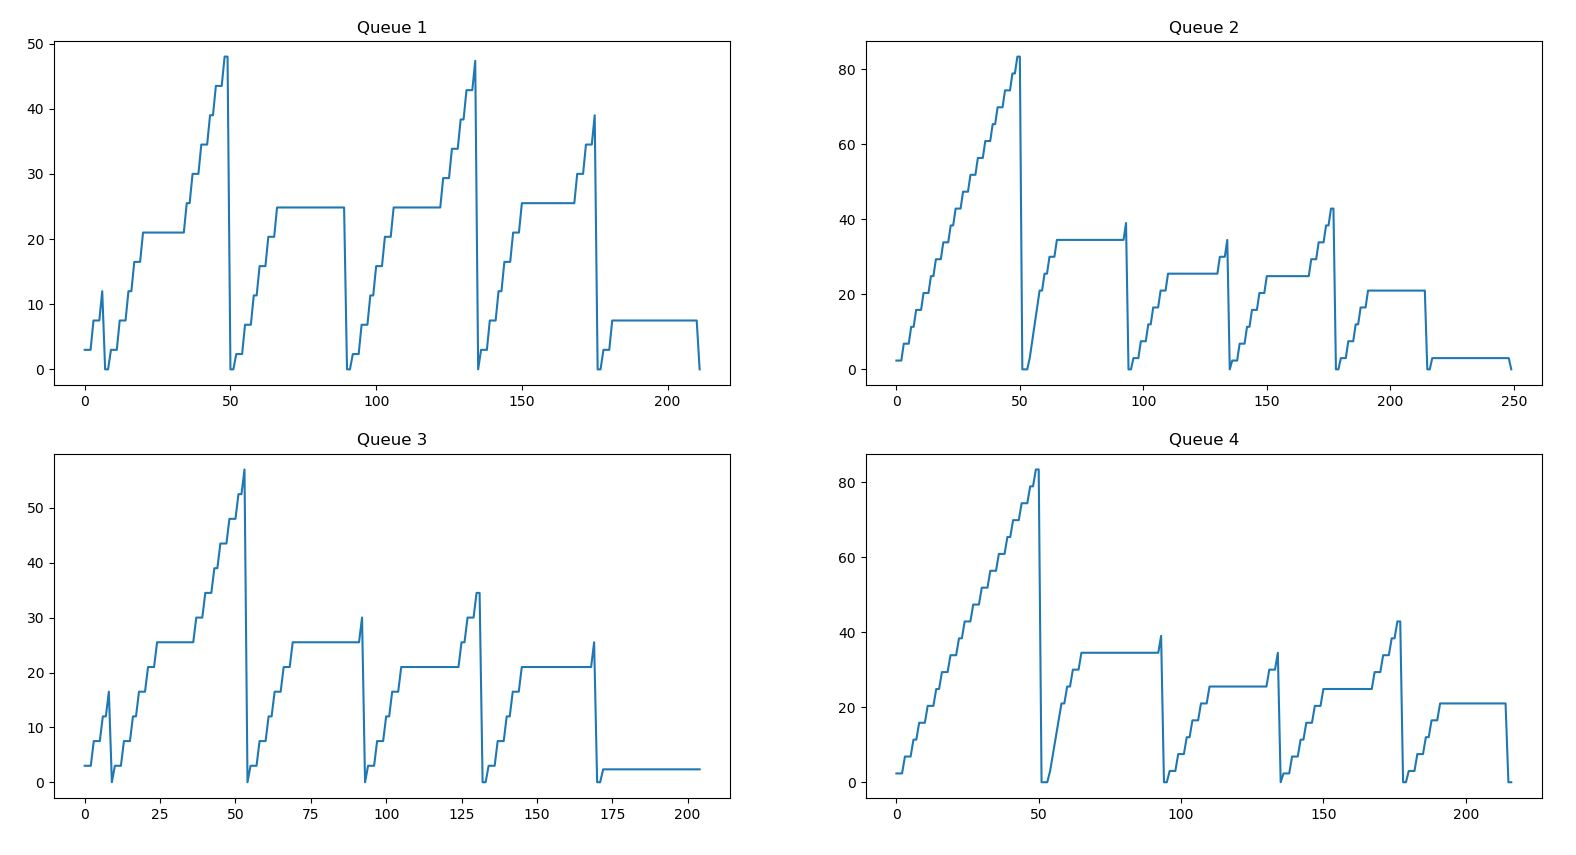
\includegraphics[width=1\textwidth]{figuras/queueDurationTL.JPG}
    \end{center}
    \caption[Duração das filas]{Com o sistema.}
    \label{queueTL}
\end{figure}

\begin{figure}[ht]
    \begin{center}
    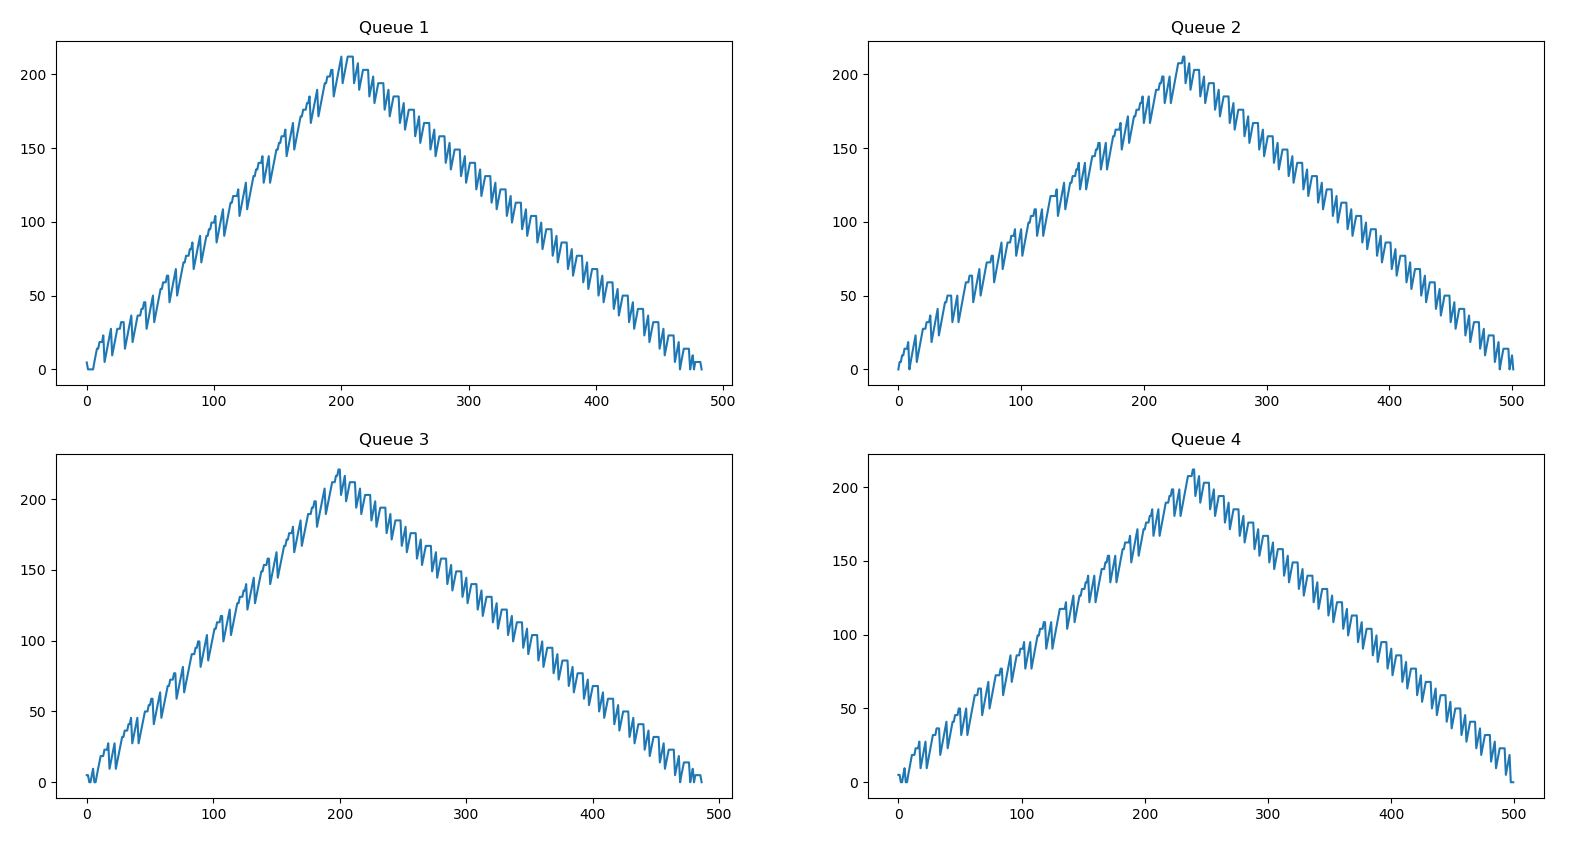
\includegraphics[width=1\textwidth]{figuras/queueDurationNoTL.JPG}
    \end{center}
    \caption[Duração das filas]{Sem o sistema.}
    \label{queueNoTL}
\end{figure}

\begin{figure}[ht]
    \begin{center}
    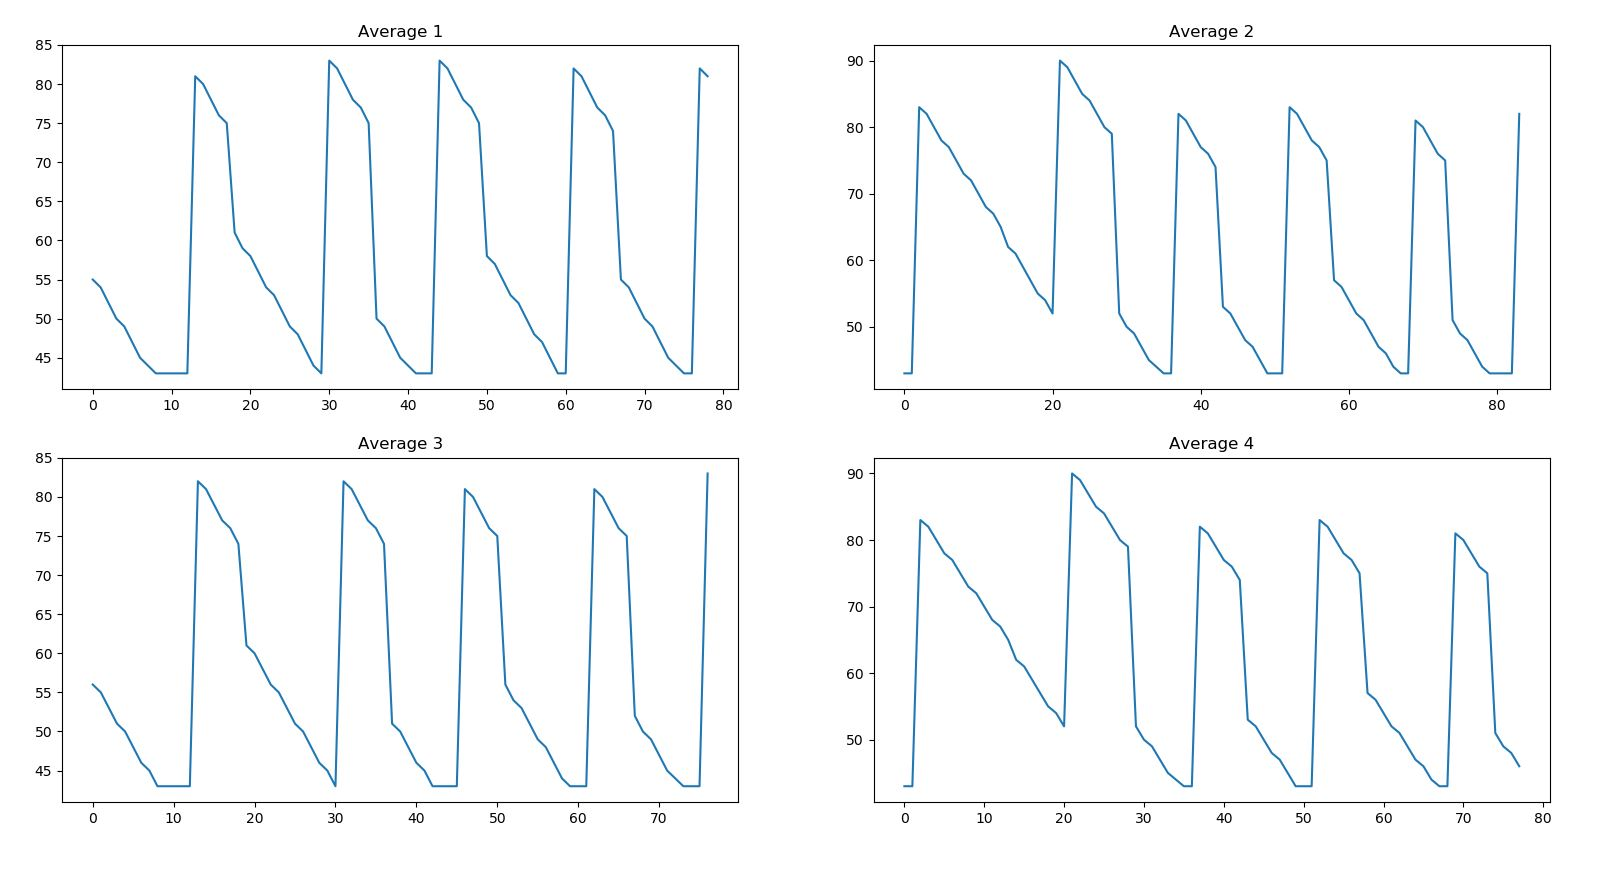
\includegraphics[width=1\textwidth]{figuras/tripDurationTL.JPG}
    \end{center}
    \caption[Duração da viagem]{Com o sistema.}
    \label{tripTL}
\end{figure}

\begin{figure}[ht]
    \begin{center}
    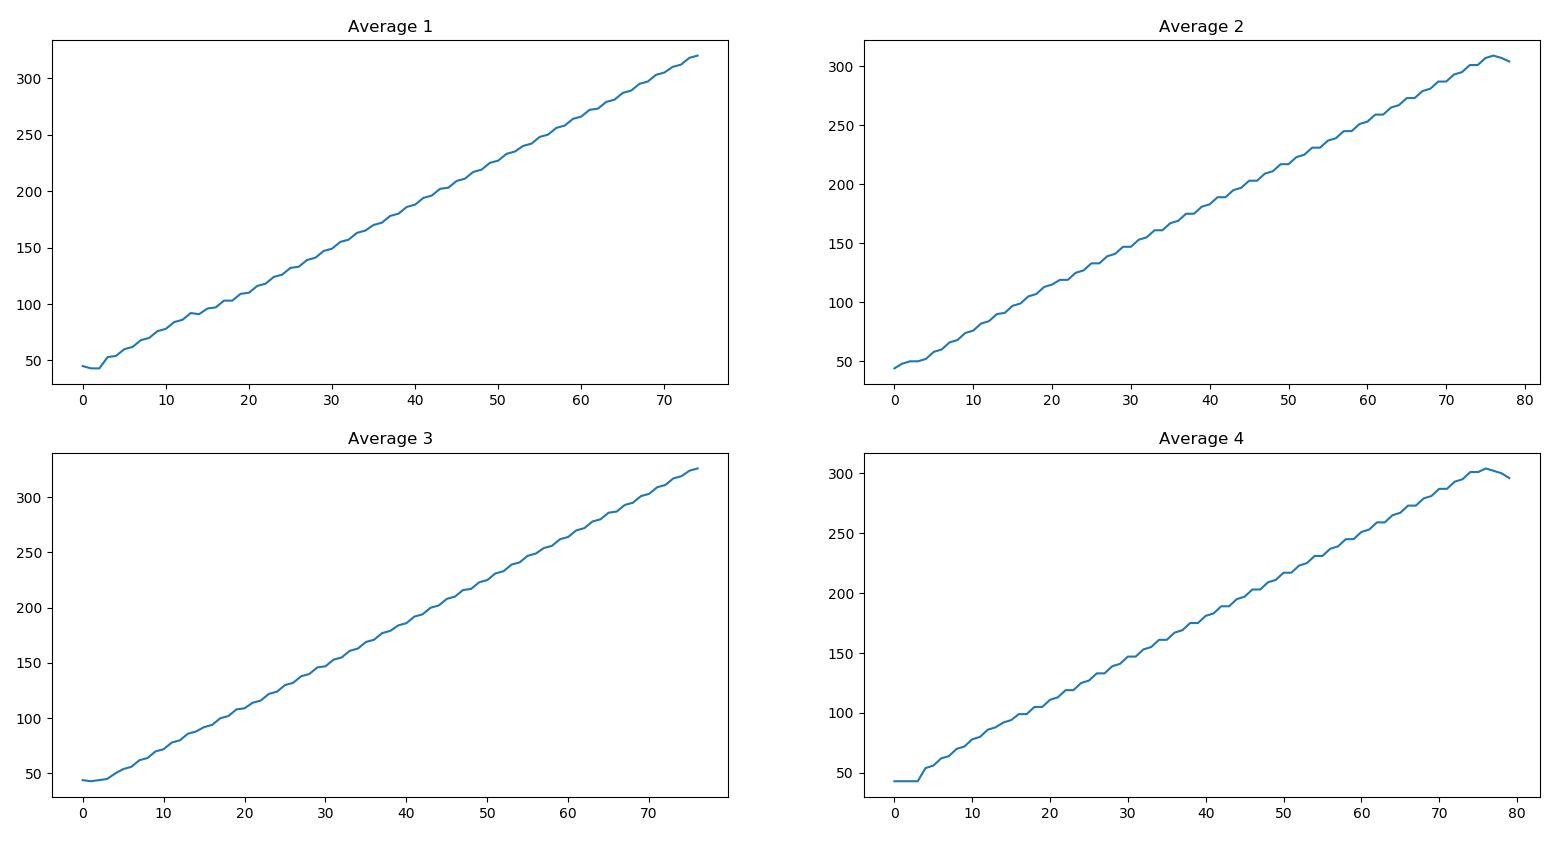
\includegraphics[width=1\textwidth]{figuras/tripDurationNoTL.JPG}
    \end{center}
    \caption[Duração da viagem]{Sem o sistema.}
    \label{tripNoTL}
\end{figure}